\section{Tekstiloome} \label{tekstiloome}
Selleks hetkeks, mil Te käesolevat malli kasutama hakkate, on Teil tõenäoliselt oma lõputöö sisuline osa valmis mõnes mugavamas ja koostöösõbralikumas keskkonnas nt Google Docs. Vormistamise juurde tasub minna siis, kui lõputöö sisuline osa enam väga ei muutu. Vastasel juhul võivad muudatused nõuda vormistamise töö uuesti tegemist. Siiski on mõned vormistusega seotud soovitused aktuaalsed ka varem kui alles mustandi puhtandiks vormistamisel.

\subsection{Peatükid}
Teie lõputöö peatükid võiksid olla üksteisega mahult tasakaalus. Kuna käesolev mall keskendub vormistamisele, siis siinkohal malli sisu selles eksib (eelnev peatükk~\ref{vormistamine} on tunduvalt mahukam kui käesolev peatükk~\ref{tekstiloome}). Teie töös võiksid kõik peatükkide “Sissejuhatus” ja “Kokkuvõtte” vahel olevad peatükid olla mahult enam-vähem võrdse kaaluga. Selline põhimõte aitab Teil ka mitte tegeleda liiga palju ainult oma lõputöö ühe osaga, vaid võrdsemalt kõigi oluliste osadega. See, mis nendes sisupeatükkides täpsemalt on ehk milliste osade vahel peaksite oma tööaega jaotama, sõltub Teie lõputöö tüübist. Tartu Ülikooli arvutiteaduse instituudis kaitstavate lõputööde nõuete ja hindamise dokument defineerib teatud arvu erineva sisu ja fookusega lõputööde tüüpe. Uurimis- või õpperühm, kus Teie oma lõputööd teete, võib defineerida neid veel omakorda. Hoidke pilk peal, et Teie lõputöö dokumendi sisu hõlmaks tasakaalukalt Teie lõputöö tüübis ettenähtavat.

\begin{wrapfigure}{r}{0.33\textwidth}
    \centering
    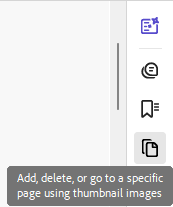
\includegraphics[width=0.33\textwidth]{figures/Joonis5-AcrobatReaderMenüü.png}
    \caption{Acrobat Reader parempoolne menüü.}
    \label{fig:acrobatReaderMenüü}
\end{wrapfigure}
Hetkel, mil Teie lõputöö hakkab vormi võtma, oleks hea vaadata lõputöö dokumenti tervikuna. Seda saab teha näiteks Acrobat Reader PDF vaaturis lehekülgede järjekorra muutmise (\emph{Add, delete, or go to specific page using thumbnail images}) tööriistaga (vt joonis~\ref{fig:acrobatReaderMenüü}). Tolle tööriista kuva näitab Teile tervet Teie tööd ülevaatlikult. Justkui oleksite oma töö välja printinud ja kõik lehed eraldi suure laua peale laotanud. Sellest ülevaatest Te näete, kas Teie erinevad töö osad on omavahel tasakaalus ja visuaalselt kooskõlas (vt joonis~\ref{fig:acrobatReaderÜlevaade}).

\begin{figure}[t]
    \centering
    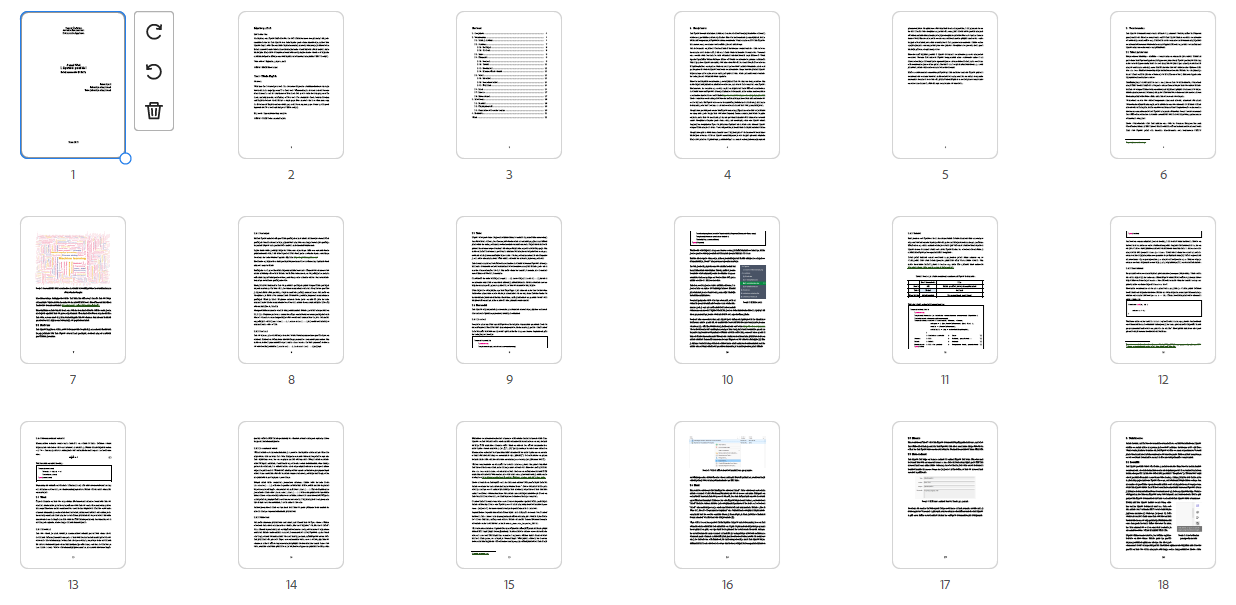
\includegraphics[width=\textwidth]{figures/Joonis6-AcrobatReaderKuva.png}
    \caption{Ülevaade lõputöö mallist Acrobat Readeris.}
    \label{fig:acrobatReaderÜlevaade}
\end{figure}
Lõputöö üldisest vaatest näeb ka, kas kõikides vajalikes kohtades on tekst olemas. Näiteks peaks iga peatükk algama peatükki sissejuhatava tekstiga. See tekst peab olema enne kui tuleb alampeatüki pealkiri. Peatükki sissejuhatav tekst kirjeldab, miks käesolev peatükk on Teie töös oluline ning mida võib lugeja oodata alampeatükkidest. Lisaks sellele võiks (alam)peatükkide sisu olla seotud omavahel siduvate lausetega ning suurema peatüki lõpus kirjas ka vastavat peatükki kokkuvõttev lõik. Peatükk ei tohiks alata ega lõppeda sisu elemendiga (joonis, tabel, koodinäide, valem) ega loeteluga. Oluline on, et Teie töö oleks sujuv lugeda.

\subsection{Õigekirjakontroll}
Puhtandi vormistamisel aitab Teid väga palju Overleafi õigekirjakontroll, mis tasub kindlasti üldmenüüst sisse lülitada ja õige keel valida. Olles mustandiga kaua aega tööd teinud, olete võib-olla juba ära harjunud ühte ja sama teksti nägema ning seetõttu võib olla raske ise kirjavigu märgata. Overleafis on olemas nii eesti kui inglise keele jaoks õigekirjakontrolli tööriist. Kirjavigadega töö korral on Teil oht saada madalam hinnang.

Muidugi võite kasutada ka teisi õigekirja parandavaid tööriistu nt Grammarly, kui Teil on neile ligipääs ja need Teie tööd efektiivsemaks teevad.

\subsection{Generatiivse tehisaru kasutamine}
Generatiivse tehisaru tööriistad ja nende kasutamine võimaldab ka Teie tööd efektiivsemaks muuta. Siinkohal keskendume tehisaru kasutamist tekstitoimetamise seisukohast. Olukorras, kus olete tehisaru kasutanud oma töö sisulistel eesmärkidel (nt uuringu küsimuste koostamisel), tuleks Teil kindlasti see kasutusmetoodika ära kirjeldada oma töö sisu osas. Seevastu teksti toimetamine ei ole Teie töö sisuline osa ja selle tarvis tehisaru tööriista kasutamist tuleks Teil lihtsalt mainida näiteks töö Sissejuhatuse peatüki lõpus.

Hea viis tehisarul põhinevat juturobotit kasutada on näiteks anda talle ette oma lõputööst lõik ja viip muuta antud akadeemilise teksti lõik paremini loetavamaks. Selle juures tuleb tulemus ise üle lugeda ja vajadusel veel korrigeerida. Tehisarul põhinev juturobot võib olla väärastanud Teie lõigus olnud mõtted ning need tuleb Teil taastada. Samuti ei pruugi Te isiklikult olla nõus konkreetse tulemuse stiiliga ning tahate seda ise veel omakorda korrigeerida. Tehisarul põhinevad tööriistad võivad aidata Teil teksti loetavust väga efektiivselt parandada, kuid Teil on vaja olla hoolas, et tehisaru poolt pakutud teksti poolt kantud mõtted on endiselt Teie ja pakutav akadeemilise stiili valik Teile meelepärane.

Kindlasti ei tasu ainult tehisaru poolt mõeldud lõike või sisu vahetult oma lõputöös kasutada. Lõputöö autor olete ikkagi Teie ning see tähendab, et Teie vastutate lõputöös kirjutatu eest. Tüüpiliselt on tehisaru kirjutatud tekst liiga üldistav, ülemäära illustratiivne ning sisaldab faktivigu, mida asjatundlik inimesest teksti autor ei teeks. Te ei taha olukorda, kus peate hakkama tekstis leiduvate probleemide pärast hakkama süüd näitama kasutatud tehisaru tööriista poole.
